\chapter{Identifying dwarf and giant color separations} \label{chap:2}
% TEXT ==========================================

We present how we go from the original Michigan Spectral Catalogs \citep{Houk1975,Houk1978,Houk1982,Houk1988,Houk1999} and filter the catalogs for ``cleaner'' spectral sub-types and luminosity classes. We also discuss how we cross-matched these cleaned Michigan targets to infrared catalogs 2MASS and WISE \citep{2MASS,ALLWISE}. By combining both infrared photometry and luminosity/spectral class information from all three sources, we are able to search for a possible color separation among dwarfs and giants of the same spectral sub-type. We remark that giant population versus dwarf population remains relatively even across galactic latitude $b$, so there should not be a dependence on sky area for color separation (see Figure \ref{fig:b-vs-count}).

\section{Combining spectral and photometric data} \label{sec:cross-matching}
We utilize the five volumes of the Michigan Spectral atlases \citep[]{Houk1975, Houk1978, Houk1982,Houk1988,Houk1999}. These catalogs characterize 150,952 HD stars over a range in B1900 declinations (Table \ref{table:michigan_pops}) for HD numbers $<$225300 (e.g., not including extensions to the HD catalog) with photographic magnitudes as faint as $\sim$9.

The spectra were exposed on objective-prism plates at the Michigan Curtis Schmidt Telescope at Cerro Tololo Inter-American Observatory. The spectra, with an average resolution of $\sim$ $2^\circ / $mm, were classified visually in spectral type and luminosity class (e.g. ``G0IV'', ``K2V'', etc.).  

We remove from the Michigan catalogs all targets with peculiar and/or mixed spectral types and luminosity classes (e.g. ``M2/3III'', ``G2e+K0V'', etc.).  The  number of targets in each Michigan Catalog with both a single spectral type and luminosity class assignment are typically $>$50\% and are listed in Table 1, with a total of $\sim$87,000 stars. We plot in Figure \ref{fig:spt_michigan_hist} the distribution of spectral types as a function of luminosity class of the ``cleaned'' sample from the Michigan Spectral Catalogs.  These histograms include the Michigan Spectral Atlas stars that do not have good positional cross-matches and photometry from 2MASS and WISE. 

All entries of the Michigan spectral atlas of HD stars were cross-matched with 2MASS \citep{Skrutskie2006} by using the SIMBAD web tool\footnote{Available at \url{http://simbad.u-strasbg.fr}} to obtain their 2MASS designations. A cross-match to AllWISE \cite{ALLWISE,ALLWISE-dwarfs} was then performed with the method described by \cite{BANYAN}. In summary, AllWISE entries within 3\arcsec of the 2MASS position were already identified in the AllWISE catalog available at the NASA/IPAC Science Archive\footnote{Available at \url{http://irsa.ipac.caltech.edu/}}. Cross-matches at further separations were performed by identifying the AllWISE entry nearest to each 2MASS position, and verifying that no other 2MASS entry is closer to the resulting AllWISE position.

As a result of our positional cross-matching vetting and photometric quality criteria, not all stars in our sample have photometric measurements in all bands, and the counts vary from color-to-color. For a given color, there are \bincount stars from the Michigan Spectral Atlas with good position cross-matches and photometry from 2MASS and WISE. There are specific limitations to our color analysis due to the scarcity of stars in some spectral/luminosity class bins, which is described in the next section, Chapter \ref{sec:color_stats}.

\section{Calculating color statistics} \label{sec:color_stats}
In this section, we review two main methods of conducting analysis of colors among dwarfs versus giant stars. For both methods, we bin stars by both (1) all available spectral sub-types in common with our cross-matched sample of \bincount stars and (2) all luminosity classes. For \ref{subsec:median_stats}, we bin by individual luminosity classes ($I$,$II$,$III$,$IV$,$V$). For \ref{subsec:tdist_stats} we bin by two separate luminosity class groups; dwarfs are specifically luminosity class $V$ and giants are all other luminosity classes ($II$,$III$,$IV$). Limitations for both analyses are mainly due to the scarcity of stars for some spectral sub-types and luminosity class bins. 

\subsection{Median and robust standard deviation} \label{subsec:median_stats}
For all photometry stated in the introduction of Chapter \ref{chap:2}, all stars that match a single spectral type and luminosity class, have good photometry measurements, and have a good positional cross-match between 2MASS and WISE, we calculate the median and robust standard deviation of stellar colors $J-H$, $J-K_{s}$, $H-K_{s}$, $J-W_{1}$, $J-W_{2}$, $J-W_{3}$, $J-W_{4}$, $H-W_{1}$, $H-W_{2}$, $H-W_{3}$, $H-W_{4}$, $K_{s}-W_{1}$, $K_{s}-W_{2}$, $K_{s}-W_{3}$, $K_{s}-W_{4}$, $W_{1}-W_{2}$, $W_{1}-W_{3}$, $W_{1}-W_{4}$, $W_{2}-W_{3}$, $W_{2}-W_{4}$, and $W_{3}-W_{4}$. When only three stars are in a given spectral type and luminosity class bin for a given color, we compute the standard deviation rather than the robust standard deviation.  When only two stars are in a given spectral type and luminosity class bin for a given color, we compute the range rather than the robust standard deviation.  When only one star has a given spectral type and luminosity class, we do not compute a distribution range.  When zero stars are in a given spectral type and luminosity class, we do not compute a distribution median.  The colors and standard deviations of the Michigan Spectral Catalogs are listed as a function of spectral type and luminosity class in Table \ref{table:color_medians}, and plotted, as an example, for \jwone and \jwtwo in Figures \ref{fig:median_stick_bar_jw1} and \ref{fig:median_stick_bar_jw2}.

\subsection{Fitting to a probability function} \label{subsec:tdist_stats}
In this section we provide an additional method of possibly identifying color separation, which is to fit color magnitudes in each spectral and luminosity bin to a Student's t-distribution function. Fitting to this type of distribution is also likely to be a more reliable method in dealing with the scarcity of stars in some bins than medians and robust standard deviations alone. As the sample size increases, a Student's t-distribution will approach a normal distribution, which is the expected behavior for the colors of stars within the same given spectral type or luminosity class.

A Student's t-distribution function is defined as the following:

\begin{equation}
    t \equiv \frac{\bar{x}-\mu}{s/\sqrt{N}} ,
\end{equation}

Where $x_{i}$ is a single experimental measurement, or color magnitude in our case. Variable $\mu$ is the population mean, $\bar{x}$ is the sample mean, and $s$ is an estimator for standard deviation $\sigma$, where $\sigma$ is not known due to small sample size $N$ \citep[student-t-citation][]{student-t}. The sample variance $s$ for a Student's t-distribution explicitly is

\begin{equation}
    s^2 \equiv \frac{1}{N-1}\sum_{i=1}^{N} (x_{i}-\bar{x})^2
\end{equation}

The assumption that we do not know the standard deviation $\sigma$ is reasonable given the very few number of stars in a non-negligible number of bins (see Table \ref{table:bin_counts} for bin counts of our total sample of $\sim$20,000 stars), and so Student's t is a reasonable choice of a statistical distribution for our color analysis.

We used the \texttt{scipy.stats.t} module\footnote{\url{https://docs.scipy.org/doc/scipy/reference/generated/scipy.stats.t.html}} to fit and calculate an average and sample variance from color data, for each spectral and luminosity group bin. After retrieving these two statistics for each bin, we are able to generate a probability function across any artificial range of color magnitudes we may choose. In order to cover most magnitude ranges for WISE/2MASS colors, we have chosen an color magnitude array that is from -0.7 to 1.8 magnitudes, with a step size of 0.025. The step size is smaller than the average WISE/2MASS photometric uncertainty of 0.10--0.15 magnitudes \citep{2MASS,ALLWISE}. 

Now that we have an estimate of color probability given a specific luminosity class and spectral sub-type, we can explore and identify a possible color separation between dwarfs and giants in Chapter \ref{chap:3}. 

% FIGURES =======================================

\begin{figure}[t] 
    \centering
    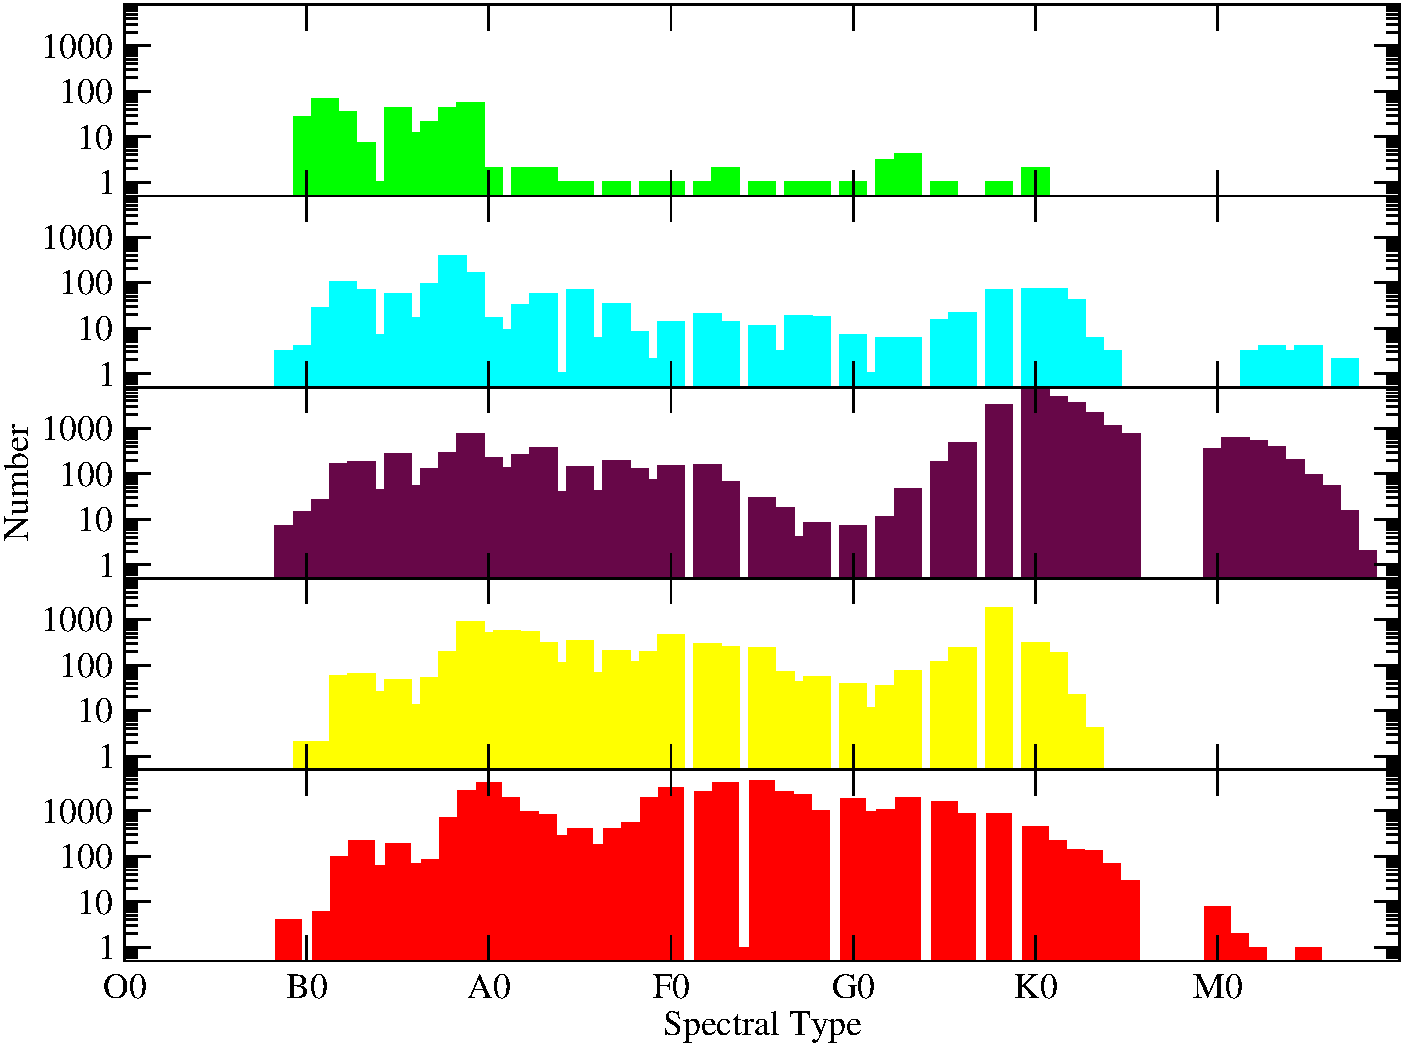
\includegraphics[width=1.0\textwidth]{Figures/populations/hist-spt-count.pdf}
\caption{The distribution of the Michigan Spectral Catalogs as a function of spectral type on the horizontal axis, after the removal of peculiar and/or mixed spectral types.  The different colors correspond to the different luminosity classes.  From bottom to top: V (red), IV (yellow), III (purple), II (cyan) and I (green).  The gaps in the histograms at particular spectral types (e.g. F1, K7-K9) indicate that this spectral type was not used for typing in the Michigan Spectral Catalogs.} \label{fig:spt_michigan_hist}
\end{figure}

\begin{figure}
    \centering
    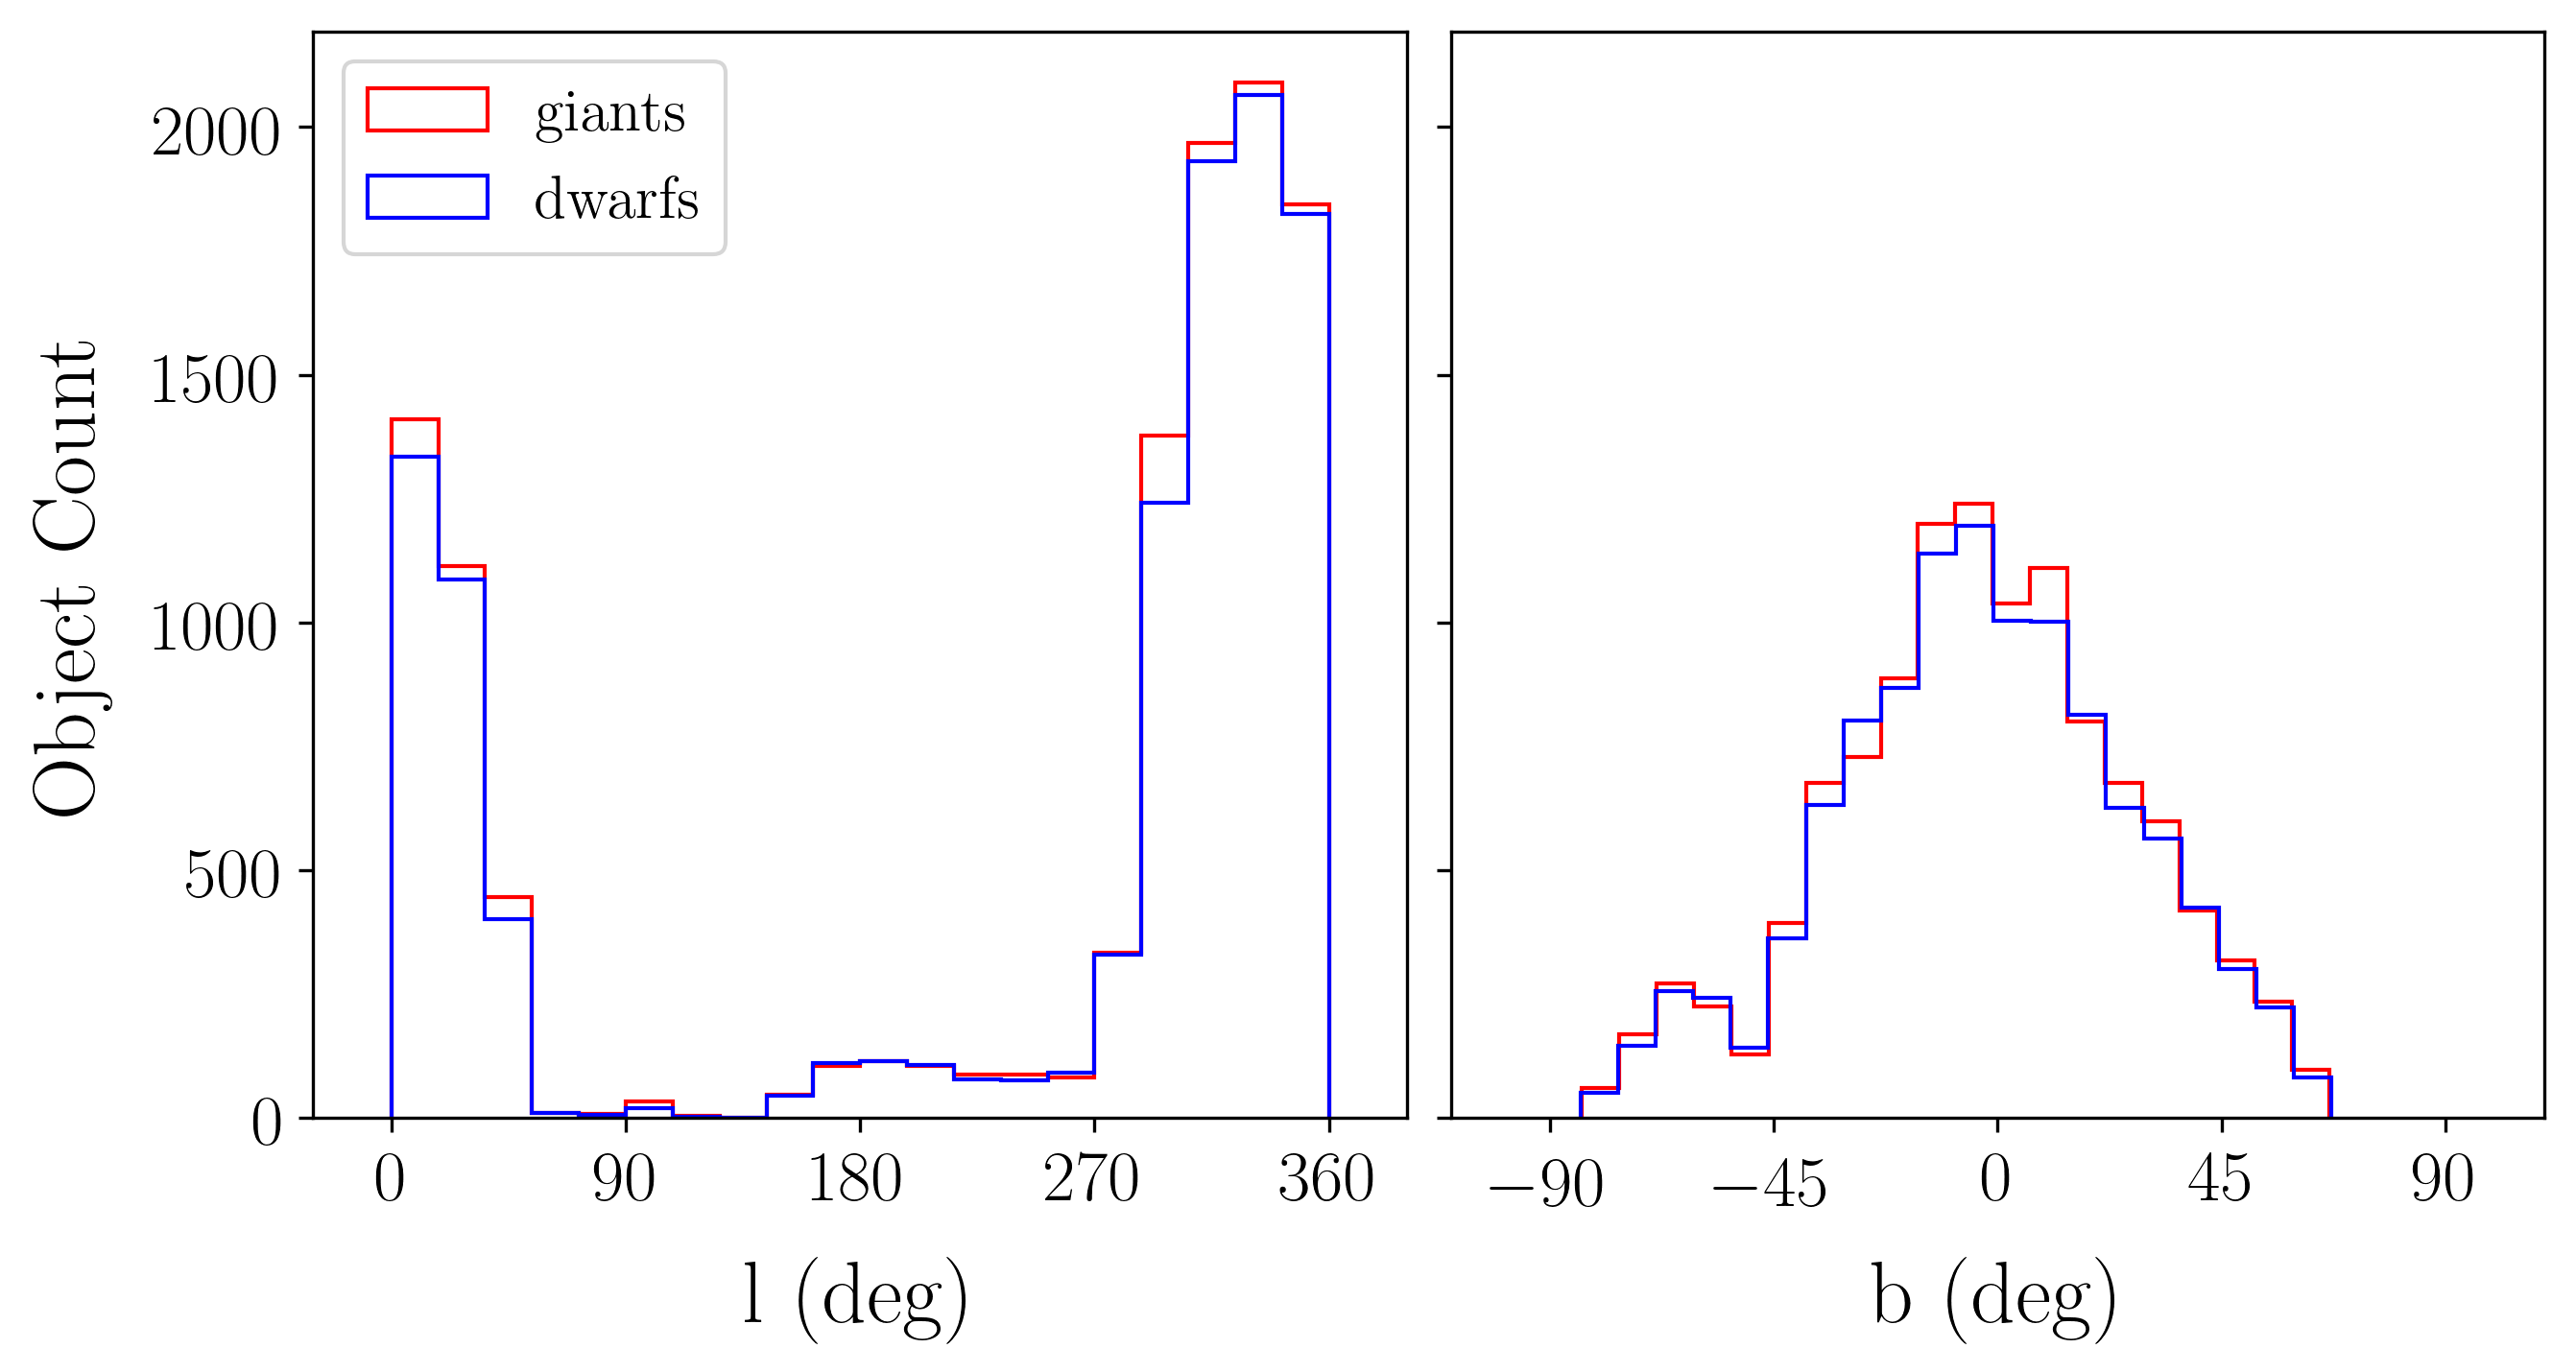
\includegraphics[width=1.0\textwidth]{Figures/populations/hist-b-vs-count.png}
    \caption{A histogram of spectra counts across all galactic latitudes ($b$) from the Michigan Spectral Atlas, which was filtered as described according to Chapter \ref{sec:cross-matching}. There is no large discrepancy of either luminosity groups.}
    \label{fig:b-vs-count}
\end{figure}

\begin{figure*}[t]
\centering
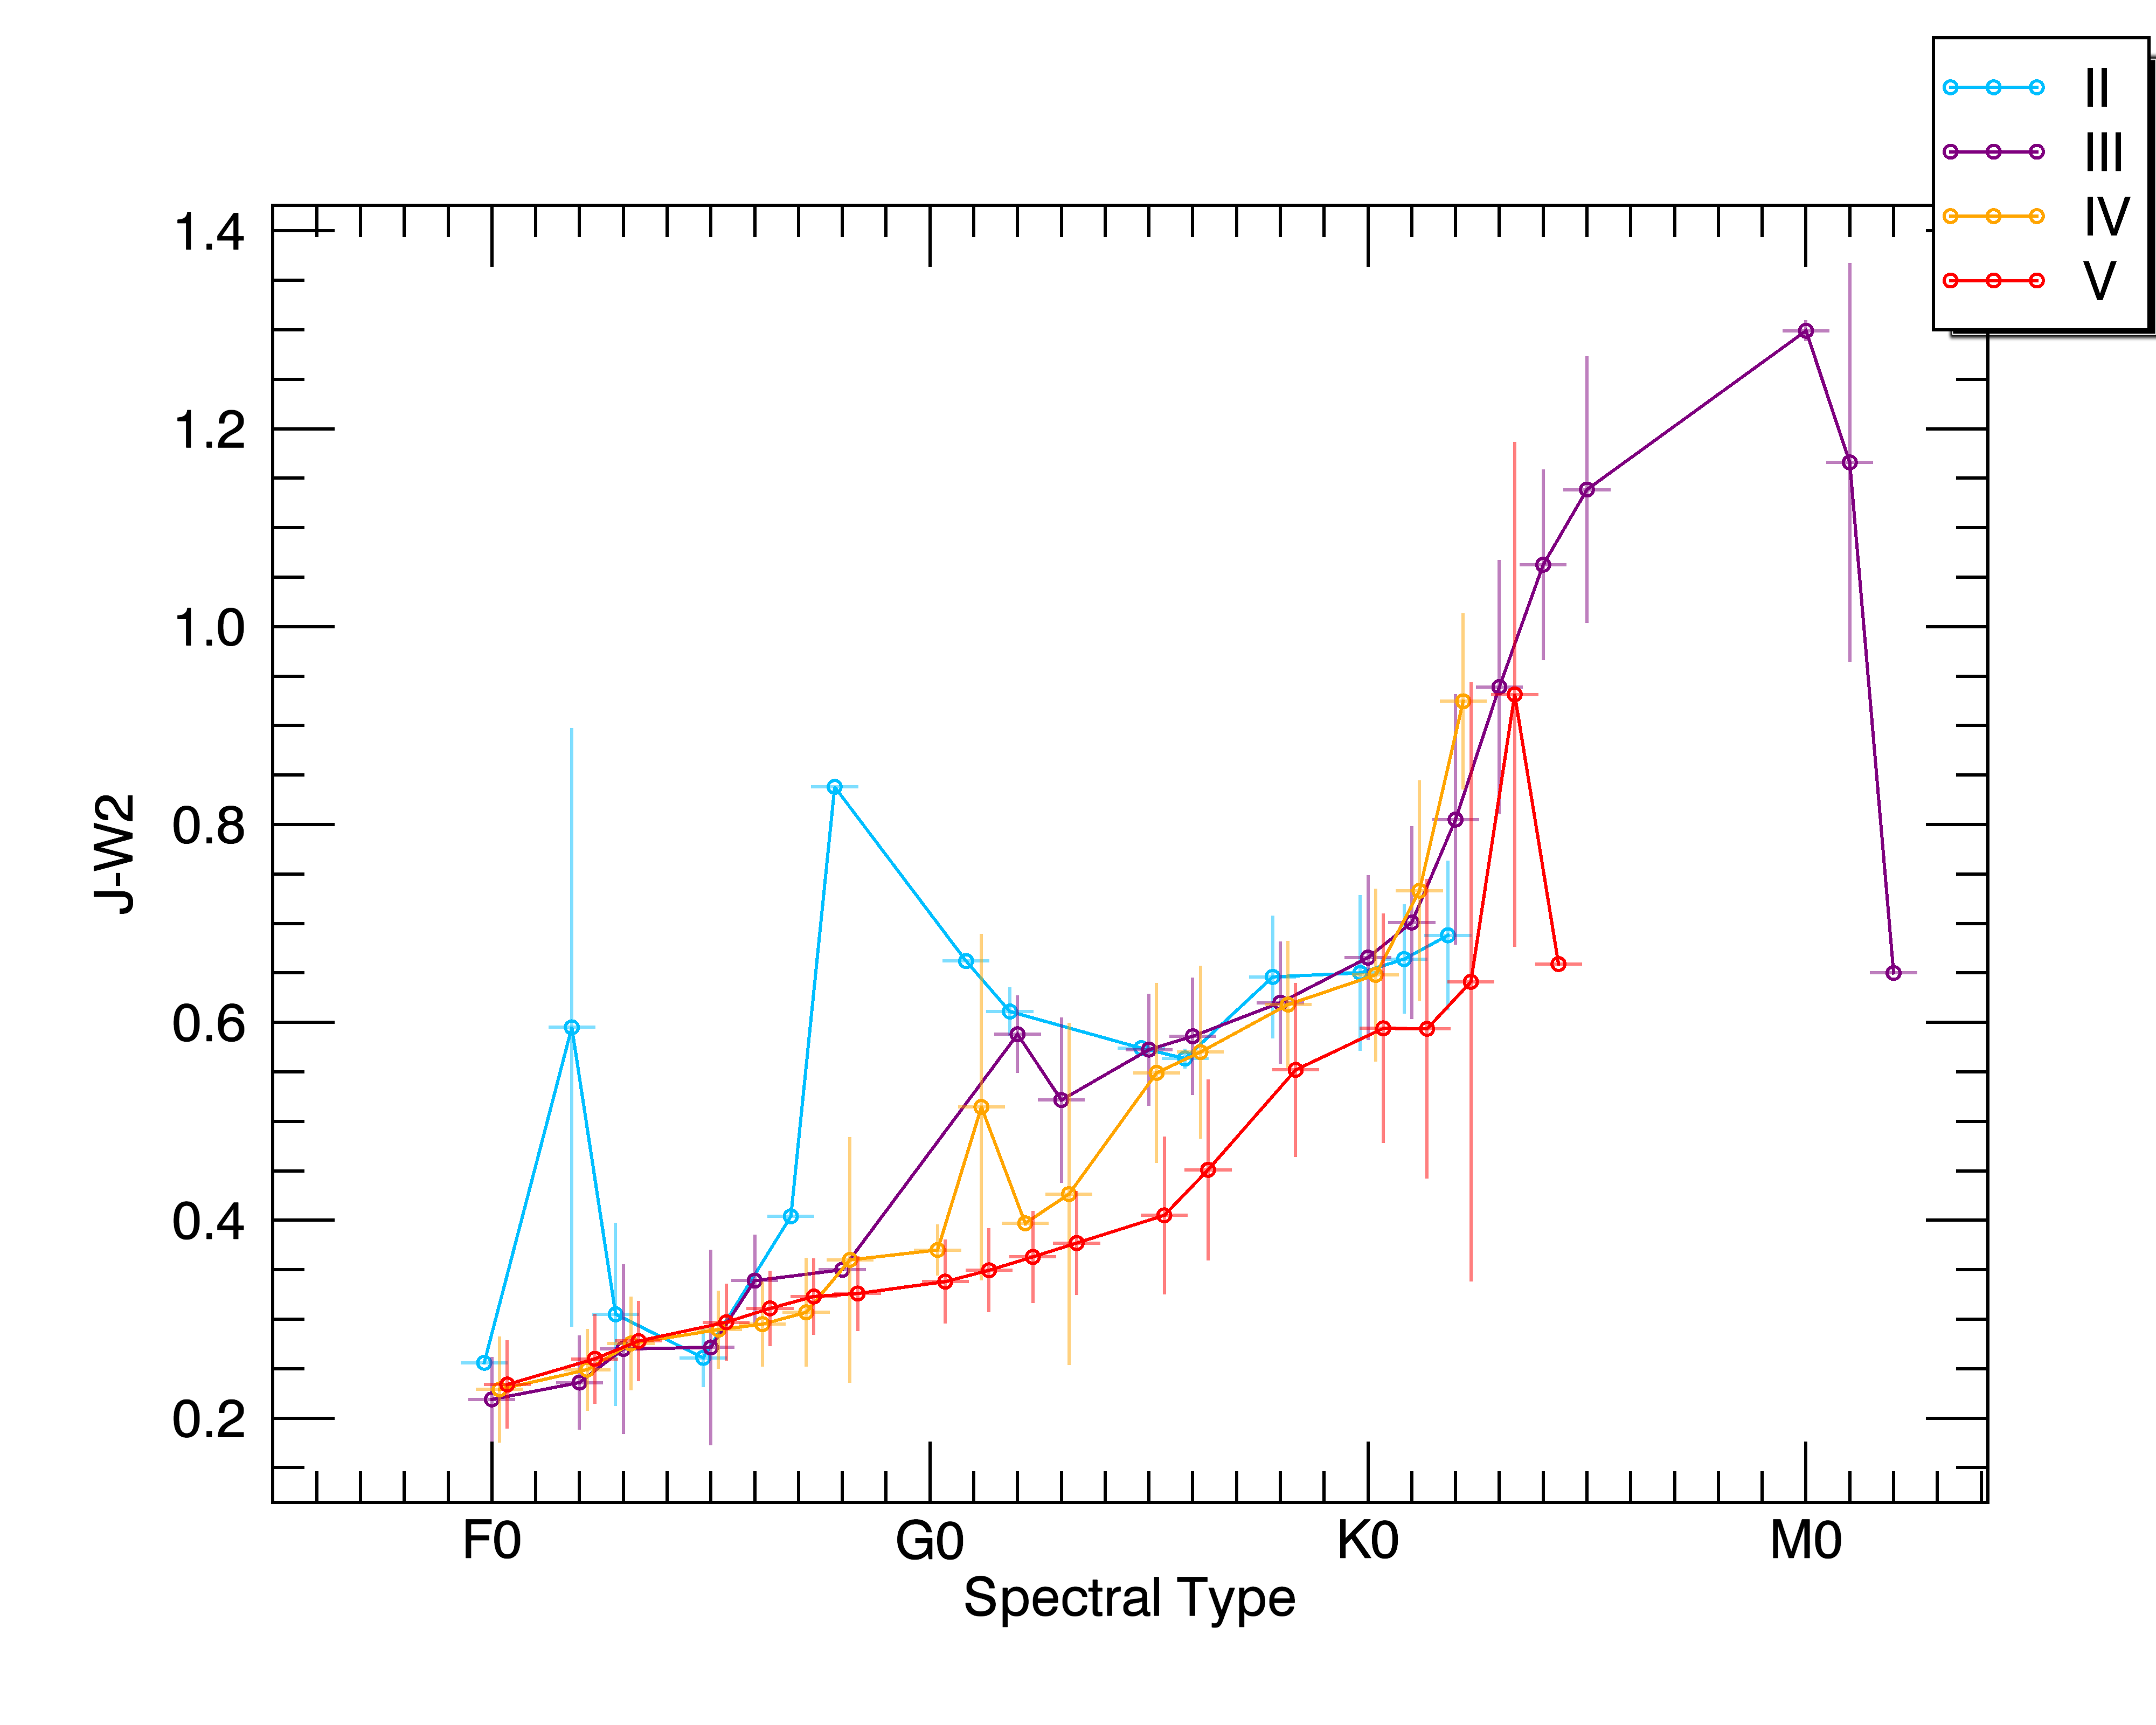
\includegraphics[width=1.0\textwidth,clip=true]{Figures/subtype_bar/SPT_J-W2.png}
\caption{The color of stars in the Michigan Spectral Catalogs as a function of spectral type on the horizontal axis, and \jwtwo on the vertical axis, after the removal of peculiar and/or mixed spectral types (see Chapter \ref{sec:cross-matching}). The different colors correspond to the different luminosity classes -- V (red), IV (yellow), III (purple), II (cyan) and I (green).  The vertical error bars generally correspond to the robust standard deviation of the \jwtwo color of stars within a given spectral type and luminosity class, unless there are only three or fewer stars, in which the error bars represent a standard deviation or range (see Chapter \ref{subsec:median_stats}, and Tables \ref{table:color_medians}). In order to see this type of figure for any other WISE and 2MASS colors as mentioned in Chapter \ref{subsec:median_stats}, see Appendix \ref{Appendix:2}.} \label{fig:median_stick_bar_jw2}
\end{figure*}

\begin{figure*}[t]
\centering
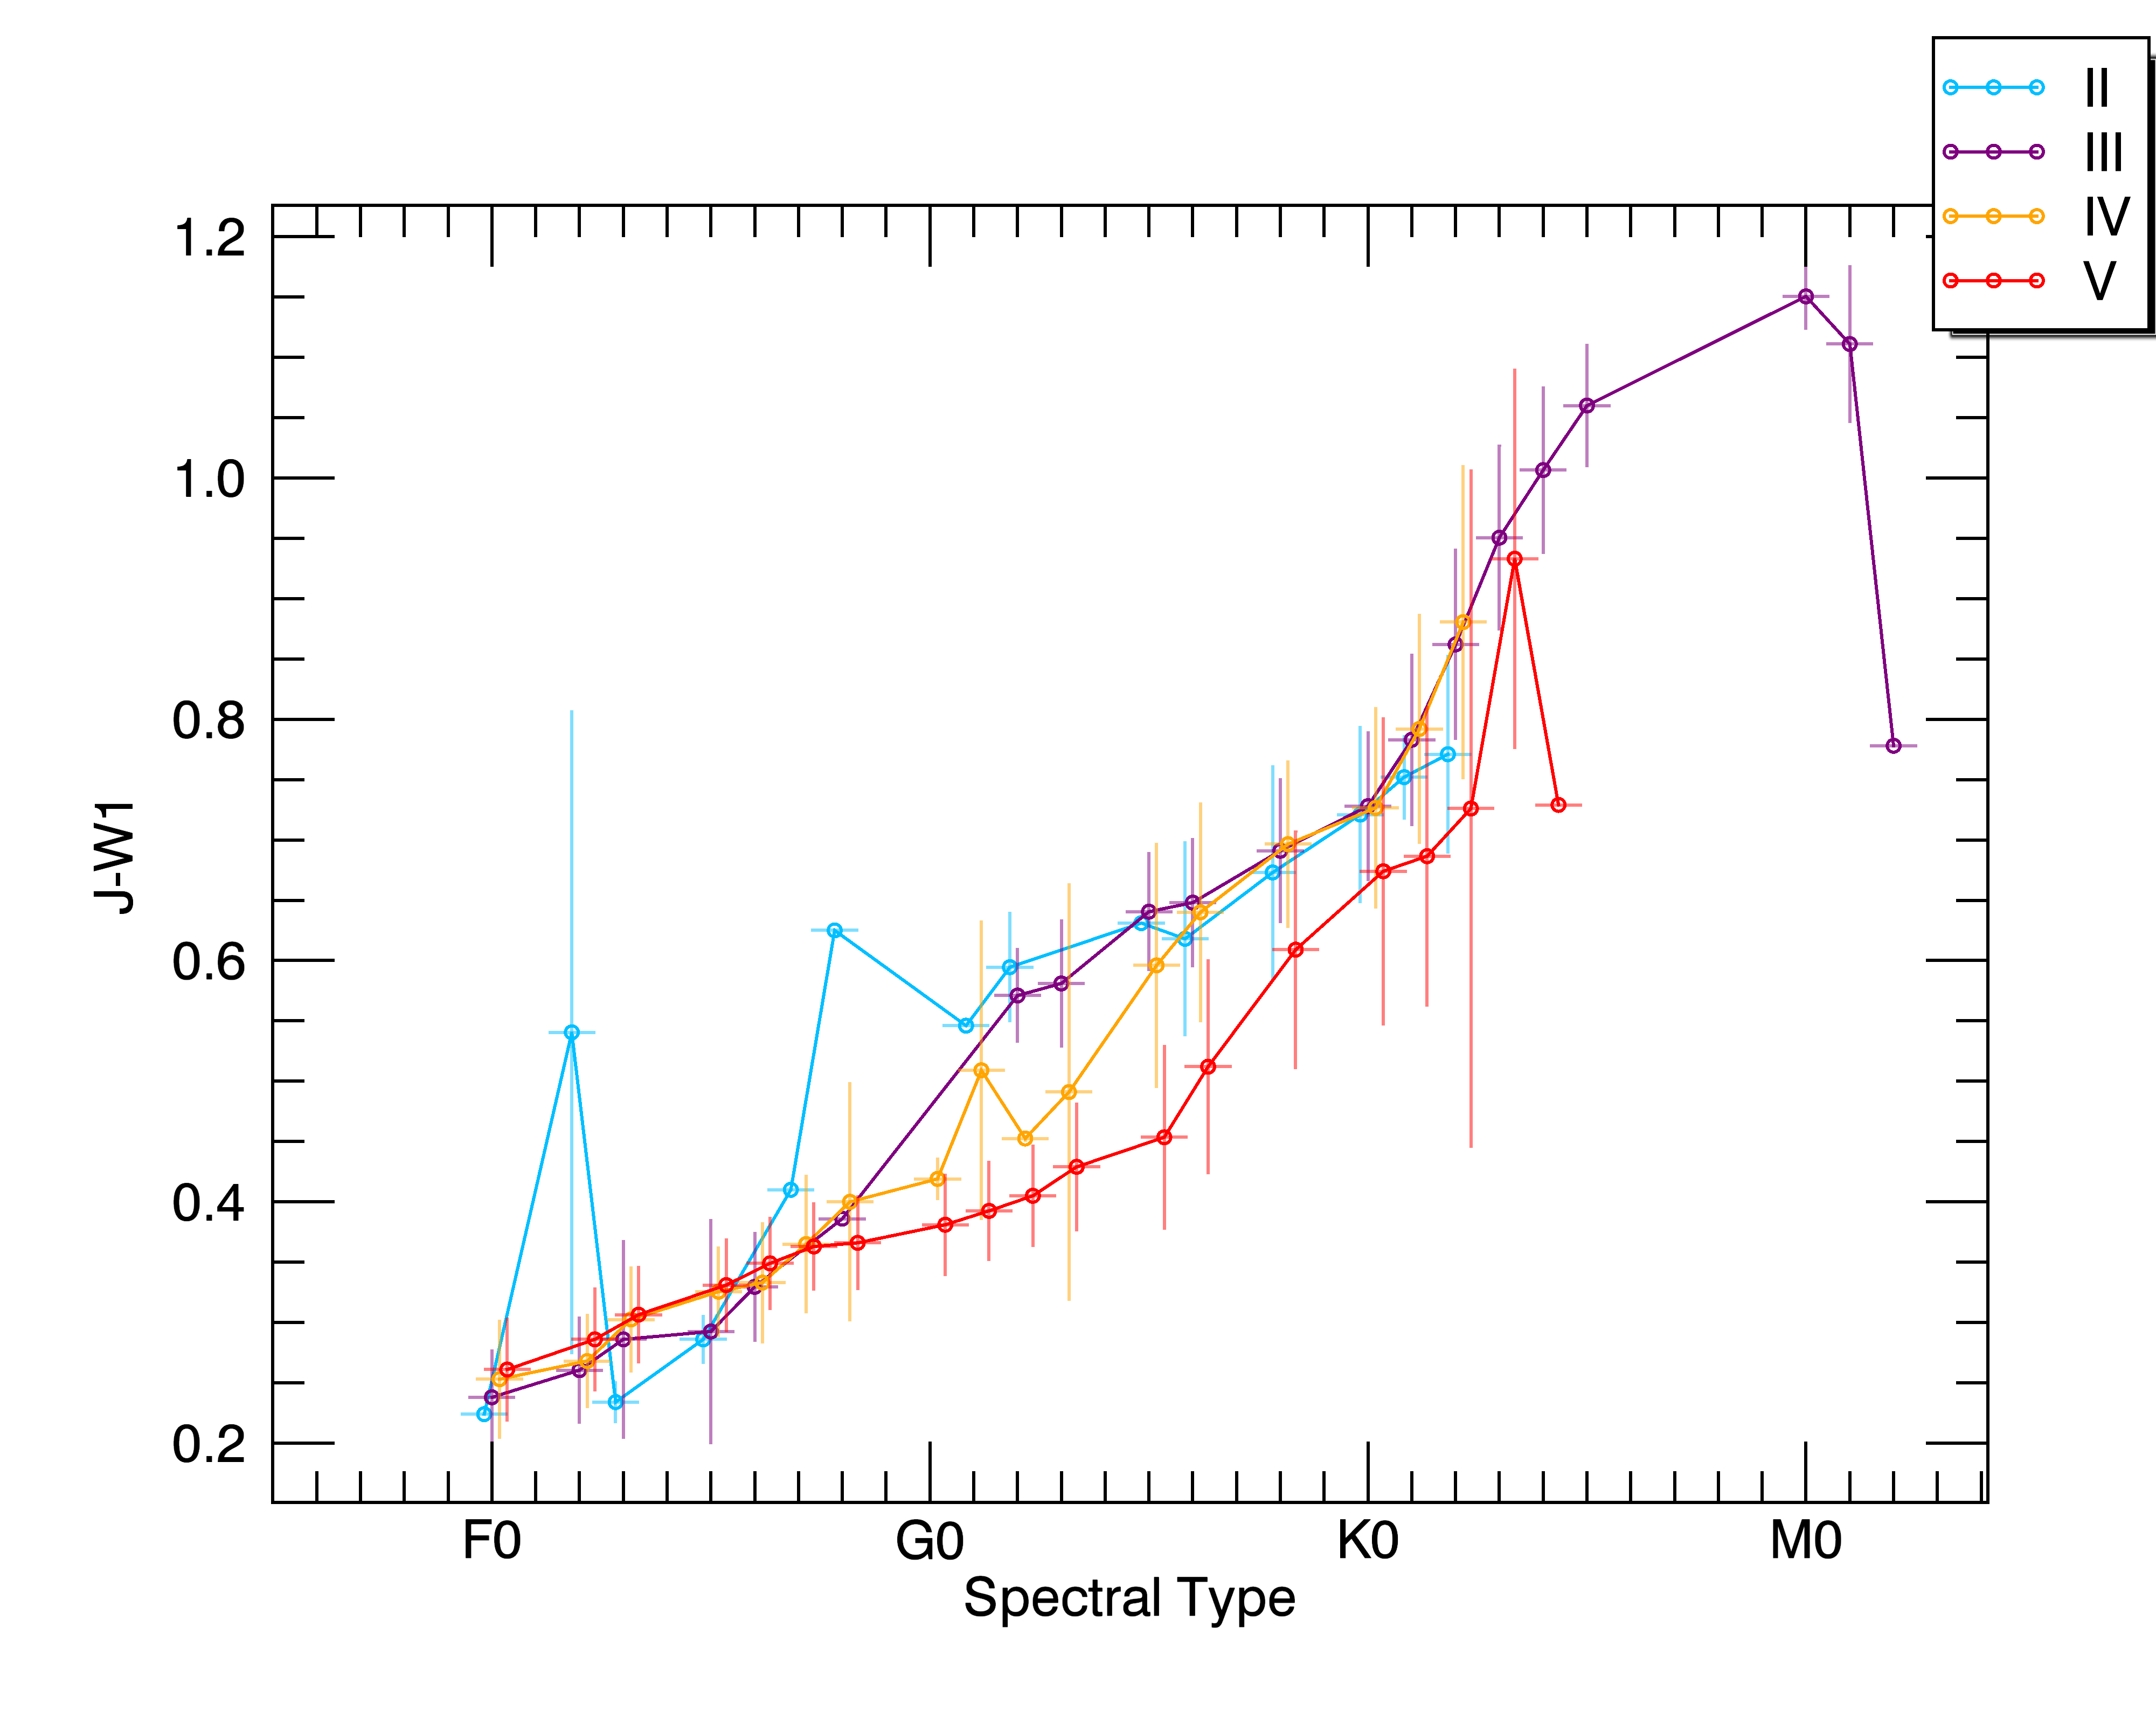
\includegraphics[width=1.0\textwidth,clip=true]{Figures/subtype_bar/SPT_J-W1.png}
\caption{Same as Figure \ref{fig:median_stick_bar_jw2}, but for $J-W{1}$.} \label{fig:median_stick_bar_jw1}
\end{figure*}